\documentclass[10pt,a4paper]{article}

% images
\usepackage[margin=1in]{geometry}
\usepackage{graphicx}
\usepackage{subfig}

\usepackage[title]{appendix}
\usepackage{pgfgantt}

% reference items
\usepackage{enumitem}

% links
\usepackage{url}
\usepackage{hyperref}

\usepackage{pdfpages}
\usepackage{pgfplots}

\usepackage{tikz}
\usetikzlibrary{arrows,automata,positioning}

\usepackage{footnote}

% maths
\usepackage{amsmath}
\usepackage{amssymb}
\usepackage{dsfont}
\usepackage{bm}

\usepackage{amsthm}

\theoremstyle{plain}
\newtheorem{theorem}{Theorem}[section]
\newtheorem{claim}[theorem]{Claim}
\newtheorem{lemma}[theorem]{Lemma}

\theoremstyle{definition}
\newtheorem{definition}[theorem]{Definition}

\newenvironment{subproof}[1][\proofname]{%
  \renewcommand{\qedsymbol}{$\blacksquare$}%
  \begin{proof}[#1]%
}{%
  \end{proof}%
}

\newtheorem*{claim*}{Claim}
\newtheorem*{corollary}{Corollary}
\newtheorem*{remark}{Remark}
\newtheorem*{fact}{Fact}

\DeclareMathOperator*{\argmax}{arg\,max}
\DeclareMathOperator*{\argmin}{arg\,min}
 
\usepackage{listings}

\lstdefinestyle{mystyle}{
    basicstyle=\ttfamily\footnotesize,
    showlines=false,
    breakatwhitespace=false,         
    breaklines=false,                 
    captionpos=b,                    
    keepspaces=false,                 
    numbers=left,                    
    numbersep=5pt,                  
    showspaces=false,              
    showstringspaces=false,
}

\lstset{style=mystyle}

\newcommand{\code}[1]{\texttt{#1}}
\newcommand*\conj[1]{\overline{#1}}
\newcommand*\vect[1]{\bm{#1}}

% No section numbering
% \setcounter{secnumdepth}{0}

\bibliographystyle{siam}

\begin{document}

\begin{titlepage}
    \begin{center}

        \vspace*{2cm}
        \includegraphics[width=.25\textwidth]{crest.png}

        \vspace*{1cm}
		{\Large \textsc{A Decentralised Peer-Prediction Market}} \\
		{\textsc{CS907 Dissertation Project - Interim Report}}

        \vspace*{1cm}
        \textbf{Thomas Archbold} \\
		1602581 \\~\\
        Department of Computer Science \\
        University of Warwick \\~\\

		\today
        % July 16, 2020 \\~\\

        \vfill

    \end{center}
\end{titlepage}

\section{Introduction}

Prediction markets are exchange-traded markets\footnote{Markets in which all
transactions are routed through a central source.} which allow users to trade
on the outcomes of future events as opposed to traditional financial
instruments. Users participate by placing bets and buying or selling shares in
various markets. Since users stake their own money the market prices should
indicate the true beliefs of the userbase and the perceived likelihood of
events occurring. Different users will have different beliefs and knowledge
informing their decisions, hence a prediction market provides a means of
aggregating information on topics of interest using ``the wisdom of the
crowd''. Securities in these markets are usually traded between \$0 and \$1,
and for binary events a market will typically pay out \$1 for every share held
for a positive outcome, and \$0 otherwise.

Traditional prediction markets are centralised in the sense that the system
provides the bets for the users to trade in, and traders simply choose at what
price point and quantity of shares to participate. Since the system knows all
possible bets beforehand it is then easy for it to be responsible for
determining the outcomes of these markets and paying out the winnings
accordingly. There are two issues with this centralised approach: firstly, it
restricts the types of bets that can be made, since they must be explicitly
offered by the market maker; secondly, it operates on trust -- there is nothing
to stop the central market maker from manipulating the system for their own
gain. We aim for a system that avoids both of these issues.

In this project we implement a \emph{decentralised} prediction market in which
it is up to the userbase itself to define the markets and determine the
outcomes of these events -- these outcomes are decided upon by consensus among
a group of users, known as arbiters. This removes the need for a trusted
centre, however with no central moderator bets may become ambiguous or their
outcomes subjective, and arbiters may still attempt to manipulate the outcome
of the market for their own gain by submitting false reports. It is also
important that users continue to act according to their true beliefs. We base
our design on the incentive compatible outcome determination mechanism proposed
by Freeman, Lahaie, and Pennock~\cite{CODiPM}.

The rest of the report is structured as follows: in
Section~\ref{sec:background} we give an overview of the current literature on
prediction markets, and in particular decentralised markets. In
Section~\ref{sec:goals} we outline the specific goals of the project and
briefly detail the current progress we have made. In Section~\ref{sec:design}
we discuss the high-level system design, tools we use, and implementation
details. In Section~\ref{sec:projectManagement} we detail the approach taken to
the project's development, ethical considerations, and scheduling issues, and
lay out plans for next tasks to complete. Finally, in
Section~\ref{sec:evaluation} we reflect on successes and failures of the
project so far.

\section{Background}

\label{sec:background}

Prediction markets receive considerable attention within the algorithmic game
theory literature. They have been used to predict the outcomes of a range of
events, particularly in business, sports, and politics~\cite{Spann2003,
Berg2006}. Nay, Van der Linden, and Gilligan~\cite{Nay2016} analyse prediction
markets empirically to study how market parameters may affect an agent's
beliefs on the real-world outcome, making the argument for a prediction market
for betting on the cause of global warming to show how increased agent
participation can cause public belief to shift towards the ``correct'' cause.
They are therefore powerful not only in aggregating public opinion, but also in
their ability to change it.

In the centralised setting Kroer, Dud\'ik, Lahaie, and
Balakrishnan~\cite{Kroer2016} introduce a cost-based market maker in which all
bets are bought and sold to the market, rather than the traders, which
sidesteps the problem of low liquidity in traditional markets. Another way to
avoid low liquidity is to use a market scoring rule: Liu, Wang, and
Chen~\cite{Liu2020} introduce Surrogate Scoring Rules to elicit private
probabilistic beliefs with access only to agents' reports, which is similar to
our setting. Their mechanisms do not rely on a ground truth to quantify the
quality of the elicited information, and could hence be particularly applicable
to decentralised prediction markets. Freeman et al.~\cite{CODiPM} take such a
decentralised approach and introduce a mechanism in which market outcomes are
crowdsourced by a group of arbiters. They derive the conditions under which
arbiters are incentivised to act truthfully, even if an arbiter reports on a
market where they themselves hold a stake, and theirs is the paper upon which
we base our design. Several other decentralised markets exist: Peterson et
al.~\cite{Peterson2015} study the setting to implement the decentralised oracle
behind the prediction market \emph{Augur}~\cite{Augur}, which uses a reputation
system to protect against manipulation. Similar markets based on
cryptocurrencies exist in \emph{Gnosis}~\cite{Gnosis} and
\emph{Hivemind}~\cite{Hivemind}, though it has not been shown that any of these
achieve any theoretical guarantees of truthfulness.

\section{Goals}

\label{sec:goals}

The overall goal of the project is to implement a decentralised prediction
market in which users may act as arbiters in markets in which they themselves
are stakeholders. This will be achieved by the following essential objectives:

\begin{itemize}
	\itemsep0em
	\item create a web application where users may specify bets to trade on
	\item implement a trading mechanism allowing users to buy and sell
		shares in user-made securities
	\item crowdsource outcome determination using reports from arbiters who may
		hold positions in the markets
	\item incentivise truthful reporting from the arbiters
\end{itemize}

These goals will largely be achieved by implementing the mechanism laid out by
Freeman et al~\cite{CODiPM}. The first three goals cover core functionality of
any decentralised prediction market, while the fourth is concerned with tuning
system parameters, before and during execution, in order to ensure that users
do not manipulate the mechanism.
 
Other features that we look to implement that are not essential to the running
of the system but highly desirable for user experience include asynchronous
communication with the server to display up-to-date pricing information without
a page refresh, and the automated closing of markets. Indeed, while their
current omission does not necessarily hamper the functionality of the market
itself, they should be implemented in order for the system to run smoothly and
independently.

The following additional features could be implemented, although they are not
the focus of the project or are unlikely to be achieved in the remaining time
frame. They include removing the need to explicitly ask for signal beliefs
from arbiters; the option to sort markets by categories; displaying user trade
histories; and sanitising database inputs.

\subsection{Progress} 

The project has so far achieved the first three goals, meaning the core
functionalities of a prediction market are implemented. Users are able to
create markets by specifying a wager and a deadline by which the outcome will
be known, and may then trade in these markets. Buying shares pushes the price
up while selling them pushes it down, both of which aggregate the perceived
likelihood of the event. Profits can be made in the markets in the traditional
way, by buying low and selling high (before the deadline has passed), or by
maintaining the position past the deadline and receiving a payout based on the
outcome of the wager.

We have also implemented crowdsourced outcome determination, in which we
resolve the outcomes of bets by collecting reports from users. These users
offer their opinion on the market's outcome, a ``yes'' or a ``no'', as well as
some extra information regarding their belief of the accuracy of their signal,
and are paid a certain amount of money as a reward for helping to resolve the
market. The payout per share is then set to the fraction of arbiters reporting
a positive result, and all users with a position are paid out, or made to buy
back shares, accordingly.

Currently, although we compute many of the values with the correct method, it
can not yet be said that we achieve truth-telling in the arbitration stage
since many of the parameters on which these values depend have been set
arbitrarily and are not yet tuned properly.

\section{Design}

\label{sec:design}

\subsection{Tools}

The project is implemented in Common Lisp and the code has been developed and
tested within the Steel Bank Common Lisp (SBCL) compiler and runtime system.
Code version control has been achieved with Git and Github.  Writing the web
application has required the use of several libraries available from the
library manager Quicklisp, specifically:

\begin{itemize}
	\itemsep0em
	\item Hunchentoot
	\item CL-WHO
	\item Mito
	\item SXQL
	\item Parenscript
	\item Smackjack
\end{itemize}

Hunchentoot provides the environment on which we host the server. Most
importantly it provides automatic session handling, allowing for multiple users
to be logged in at once, and easy access of GET and POST parameters, enabling
interaction via HTML forms. To generate the webpages, we use CL-WHO, which
converts Lisp statements into strings of valid HTML. Defining webpages while
remaining in the Lisp environment means we may use Lisp's macro system to build
abstractions for both defining structure and processing data in one interface.

Mito and SXQL provide the ability to connect to and interact with a Relational
Database Management System (RDBMS). We use MySQL, though this choice is largely
immaterial given our simple requirements of the database.

Parenscript incorporates Javascript into the site with the goal of improving
user experience. Currently it is only used to ensure that all necessary fields
during market creation, trading, and market resolution are non-empty to avoid
sending incomplete data to the server. It will be used to a greater degree in
the future to ensure responsiveness: all information displayed to the user must
be current to ensure that users are interacting with an up-to-date state of the
system. We therefore plan to make more use of Parenscript and Smackjack, an
AJAX library for Lisp, to allow for asynchronous interaction with the server.
This will include, for example, continuously updating a stock's price or
calculating the cost of a transaction without a page refresh, and stronger
client-side validation.

\subsection{System Overview}

We implement the mechanism for peer prediction introduced by Freeman et
al~\cite{CODiPM}. In this section we will introduce the main ideas they present
and give an overview of the mechanism itself.

We are interested in setting up a prediction market for the outcome of the
binary event (random variable) $X \in \{0,1\}$. The terms ``market'' and
``security'' are used interchangeably to refer to the entity comprising a wager
(e.g. ``Arsenal will beat Tottenham'') and a deadline -- these two pieces of
information are all we need to represent event $X$. The mechanism is divided
into two main stages: the market stage, where users may buy and sell shares in
the securities whose deadlines have not yet passed; and the arbitration stage,
where a subset of the users report on the outcome of the security and we
compute the payout price per share held. A key feature of this mechanism is
that users may act as arbiters in markets in which they themselves hold shares.

Since we rely heavily on user participation for the mechanism to run correctly,
it is important that users act in the desired manner. This mechanism
incentivises truthful reporting in the arbitration stage, whereby it is in a
user's best interests to report what they truly believe a market's outcome to
be and not attempt to manipulate the system, even if the user is a stakeholder
in the market. It also allows us to achieve certain guarantees, such as a bound
on the amount we must pay to arbiters to reward them for participation, which
serves as a guide when setting system parameters.

\subsubsection{Market Stage}

The market stage allows users to create markets for any event they wish and
trade shares in these markets. Since we crowdsource outcome determination,
there is no restriction placed on the types of bets users may make other than
that their result is a ``yes'' or a ``no''. Ambiguous bets are allowed, though
likely to suffer in the arbitration stage, since users may have different
interpretations on the outcome.

In order to create a market for a user-specified event, we use a \emph{market
scoring rule (MSR)}, which is a means of assigning a probability to a set of
mutually outcomes. After the wager and deadline have been specified, the MSR
simply takes into account the number of shares bought and sold and returns a
probability $p \in [0,1]$. This describes the perceived likelihood amongst
users of the event having a positive outcome. We can also use this to set the
share price of the security.  Using a MSR is different from a traditional
market in that there is not a fixed number of shares in circulation: instead,
buying into a market increases the total number of shares and selling decreases
it. Let $q$ denote the total number of shares of a given security. An agent
wishing to buy $q'-q$ shares (i.e. increasing the total number of shares to
$q'$) will pay $C(q')-C(q)$, for our choice of convex, differentiable,
monotonically increasing scoring rule $C$. We may tune the behaviour of this
cost function by using a liquidity parameter $b$, such that $C_b(q) := b \cdot
C(q/b)$, which controls the responsiveness of $C$. A lower value of $b$ means
that the share price changes more quickly for fewer shares bought, and vice
versa.

The market stage implements trading fees in order to raise the funds necessary
to pay stakeholders when the event's outcome is realised, and to reward users
for participation in the arbitration stage. Buying shares pushes the share
price $p$ towards \$1, while selling shares pushes it towards \$0, and the fee
can be interpreted as a fee on the worst-case loss that an agent incurs. For a
fixed parameter $f$, a ``buy'' transaction that pushes the share price to $p$
incurs an additional charge of $fp$, while a ``sell'' transaction incurs a
charge of $f(1-p)$. Transactions are only charged a fee when the user increases
their risk: if they are simply liquidating their position (selling shares they
own or buying back shares they have sold) then no fee is charged.  Users may
trade in the market as long as they have enough funds to make the transaction
and the deadline for the event has not passed. After the deadline has expired
the users' positions are final and we move on to determining the outcome of the
event in the arbitration stage.

\subsubsection{Arbitration Stage}

The arbitration stage is concerned with determining the perceived outcome of
event $X$ by taking reports from a subset of the users in the system, known as
the arbiters. Each arbiter $i$ receives a (private) signal $x_i \in \{0,1\}$
that tells them the result of the event -- this is analogous to reading the
news, watching the match, or even hearing about it from a friend. They then
submit a report $\hat{x}_i \in \{0,1\}$ to the system that tells us what they
believe the outcome to be. Note that since the signal they receive is private,
we have no way to know whether the user is reporting what they truly believe,
or whether they are trying to manipulate the system for their own gain.
Arbiters are then paired randomly, and paired arbiters $i$ and $j$ are paid a
reward of $u(\hat{x}_i, \hat{x}_j)$ according to the ``1/prior with midpoint''
mechanism, which we will detail below.

We can now determine the outcome of the market. In a traditional prediction
market, users are paid \$1 for each share owned (or they must buy shares back
at \$1 if they have shorted the security) if the event has a positive outcome,
and \$0 otherwise. Hence if an event is almost certain to occur, more users
will buy shares than sell them, as they expect they will be paid out for
holding shares in the market when the outcome is realised. This will push the
share price towards \$1. Similarly, if an event is believed to be unlikely,
more users will sell shares than buy them and the price will approach \$0. This
prevents arbitrarily large profits being made for risk-free bets. In our market
the outcome of an event is the random variable $\hat{X} \in [0,1]$ which is set
to the proportion of arbiters that submit a report of $\hat{x}_i=1$.
Stakeholders are then paid out in the usual way.

\subsubsection{1/prior mechanism}

\label{sec:oneOverPrior}

We use the 1/prior payment mechanism to reward users for submitting reports on
the outcomes of events, with a modification to incentivise truthful reporting.
The 1/prior payment mechanism was conceived by Jurca and
Faltings~\cite{JurcaFaltings2008, JurcaFaltings2011} as a means of rewarding
arbiters for participation in opinion polls, and Witkowski~\cite{Witkowski2014}
generalises this mechanism to pay out different amounts depending on the
signals reported by paired arbiters. For paired arbiters $i$ and $j$ with
reports $\hat{x}_i$ and $\hat{x}_j$, the 1/prior mechanism pays $i$ and $j$ as
a reward for reporting on the market outcome:
%
\begin{equation}
	\label{eq:oneOverPrior}
	u(\hat{x}_i, \hat{x}_j) =
	\begin{cases}
		k \mu & \text{if } \hat{x}_i = \hat{x}_j = 0 \\
		k (1-\mu) & \text{if } \hat{x}_i = \hat{x}_j = 1 \\
		0 & \text{otherwise}
	\end{cases}
\end{equation}
%
in which $k$ is a parameter and $\mu$ is the (common) prior belief that $X=1$.
A suitable value to use for $\mu$ would be the closing price for the market: if
users feel an event is likely to happen the share price will be pushed towards
\$1, while if they feel it is unlikely it will be pushed towards \$0.

The modification to the 1/prior mechanism is simple though requires two extra
values to be computed. Let $\mu_1^i$ be the probability that, given that agent
$i$ receives a positive signal, another randomly chosen agent also receives a
positive signal, and let $\mu_0^i$ be the probability that, given that agent
$i$ receives a negative signal, another randomly chosen agent receives a
positive signal. We require the ``update'' probabilities $\mu_1, \mu_0$ to be
common across all agents, which we can achieve by simply taking:
%
\begin{equation}
	\begin{gathered}
		\mu_1 := \min_i \mu_1^i \\
		\mu_0 := \max_i \mu_0^i
	\end{gathered}
\end{equation}
%
The modified payment method we use, the ``1/prior with midpoint'' mechanism, is
now simply Equation~\ref{eq:oneOverPrior} with $\mu$ replaced by $(\mu_1 +
\mu_0)/2$. This guarantees the incentives for arbiters are the same regardless
of their signal.

\subsection{Implementation}

As discussed, we have currently implemented both stages of the mechanism but
are yet to tune the parameters required to achieve the truth-telling behaviour
we desire. The system comprises four independent parts, each implementing a
separate area of functionality, as follows:

\begin{enumerate}
	\itemsep0em
	\item Database
	\item Trading
	\item Arbitration
	\item Server
\end{enumerate}

\subsubsection{Database}

The database is implemented using the Mito library provided by Quicklisp. This
is an object relational mapper that provides support for MySQL, PostgreSQL, and
SQLite3. We can therefore define and interact with tables while staying
completely within the Lisp ecosystem, leading to a quicker and more flexible
development cycle.

We use three tables: \code{USER}, which stores all users in the system and
their remaining budget; \code{SECURITY}, which stores the wager, deadline,
number of shares, and outcome of every user-created security; and
\code{USER-SECURITY}, which is responsible for the many-to-many relationship
between users and securities (i.e., each user may own shares in many
securities). The latter allows us to store a user's position within a market as
well as how they report on it during the arbitration stage, if they indeed
decide to do so. The tables contain the following columns:

\begin{table}[ht]
	\centering
	\begin{tabular}{|c|c|c|}
		\hline
		\textbf{User} & Name & Budget \\ \hline
	\end{tabular} \\~\\

	\begin{tabular}{|c|c|c|c|c|}
		\hline
		\textbf{Security} & Bet & Shares & Deadline & Outcome \\ \hline
	\end{tabular} \\~\\

	\begin{tabular}{|c|c|c|c|c|c|c|}
		\hline
		\textbf{User-security} & User & Security & Shares & Report & Positive Belief & Negative Belief \\ \hline
	\end{tabular} \\~\\
\end{table}

An entry in the \code{USER} table consists of a username and a budget. There is
currently no requirement to enter a password to log in to the system -- this
has been done to speed up the testing process, and will be an easy addition in
the future.

The columns in the \code{SECURITY} table contain all information to define a
market in which users may trade: ``bet'' holds the wager that is being
proposed, ``shares'' holds the number of shares which have been bought and
sold, ``deadline'' holds the earliest date-time by which users can receive a
signal on the wager's outcome, and ``outcome'' holds the payout price per share
of the market, to pay out stakeholders.

An entry in the \code{USER-SECURITY} table stores the relationship between
users and securities, whether this is the number of shares a user holds in a
security, an arbiter's report on a security, or both. The ``user'' column
holds the user ID, ``security'' holds the security ID, and the number of shares
owned and their report (or NULL) are stored in the corresponding columns. The
columns ``positive belief'' and ``negative belief'' store a user's estimations
that, given they the event has a positive (respectively negative) outcome, they
receive a positive signal. The manner in which this is used is detailed in
Section~\ref{sec:arbitration}.

Defining such tables using Mito is as simple as using the \code{deftable}
macro, and is syntactically similar to defining a regular struct within Common
Lisp. Listing~\ref{lst:deftable} shows how we define the columns and their
associated datatypes. The macro defines default accessors\footnote{Functions
for accessing members of a struct.}, the slots \code{created\_at},
\code{updated\_at}, and a primary key \code{id} if none is specified. Insertion
is similarly straightforward: to insert a new entry into a table we create an
instance of the class that is implicitly defined when calling \code{deftable},
then call \code{create-dao}. To retrieve records from the database we use
either \code{select-dao}, which returns all records matching the conditions, or
\code{find-dao}, which returns only the first.

\begin{lstlisting}[
	label={lst:deftable},
	language=lisp,
	captionpos=b,
	caption={Defining a table in Mito}]
(deftable security ()
    ((bet :col-type :text)
     (shares :initform 0
             :col-type :integer)
     (deadline :col-type :datetime)
     (outcome :col-type (or :double :null))))
\end{lstlisting}

\subsubsection{Trading}

Trading allows users to create arbitrary bets on binary events and then trade
shares in them. It also implements the trading fees on risk transactions
required to raise funds to reward arbiters and pay out stakeholders. To
calculate the trading fee, we first need to know whether the user is increasing
their risk (a ``risk transaction'') or they are simply liquidating a position
they already hold, and secondly whether they are buying or selling shares,
since these incur different charges.

To create markets, quote their share prices, and compute the cost of a
transaction we use a market scoring rule. We use the commonly used Logarithmic
Market Scoring Rule (LMSR), created by Robin Hanson~\cite{LMSR}. As we have
mentioned, in any MSR an agent wishing to purchase $q'-q$ shares of a given
security must pay $C(q')-C(q)$ for convex, differentiable, monotonically
increasing function $C$. In the case of LMSR, for current number of shares $q$
and liquidity parameter $b$, this function is:
%
\begin{equation}
	\label{eq:LMSR}
	C_b(q) = b \log (1 + e^{q/b})
\end{equation}
%
This function also accommodates selling shares, in which case $q'<q$.  Since a
user must specify a desired amount of shares to buy or sell before we can
determine how much to charge them, we cannot use this function to directly
quote a share price. Instead, we can calculate the cost of the transaction were
the user to purchase a miniscule quantity of shares and quote this as the share
price. This is simply the derivative of Equation~\ref{eq:LMSR} and is given by:
%
\begin{equation}
	\label{eq:LMSRprice}
	p_b(q) = \frac{ e^{q/b} }{ 1 + e^{q/b} }
\end{equation}
%
Although Equation~\ref{eq:LMSRprice} quotes the share price, it is not accurate
to use it to calculate how much an agent should pay, since the agent's
participation in the market will immediately change this price. It does,
however, provide a useful means of describing to the user the perceived
likelihood of the event. For example for some security, at $q=0$ an equal
number of shares have been bought as have been sold, meaning the userbase as a
whole is equally unsure about whether the market will have a positive or
negative outcome. The quoted share price will be $p(0)=\$0.50$.  Similarly,
suppose $b=10$ and $q=20$, meaning twenty more shares have been bought than
sold in the market. This would yield a share price of $p_{10}(20) \approx
\$0.88$. Users feel more confident that the event will have a positive outcome,
since more people have bought shares, giving a higher share price. As mentioned
in Section~\ref{sec:oneOverPrior}, we interpret the closing price of the market
as the probability of a positive outcome, as it approximates how sure users
feel about the event's outcome.

\begin{figure}[h]
	\centering
	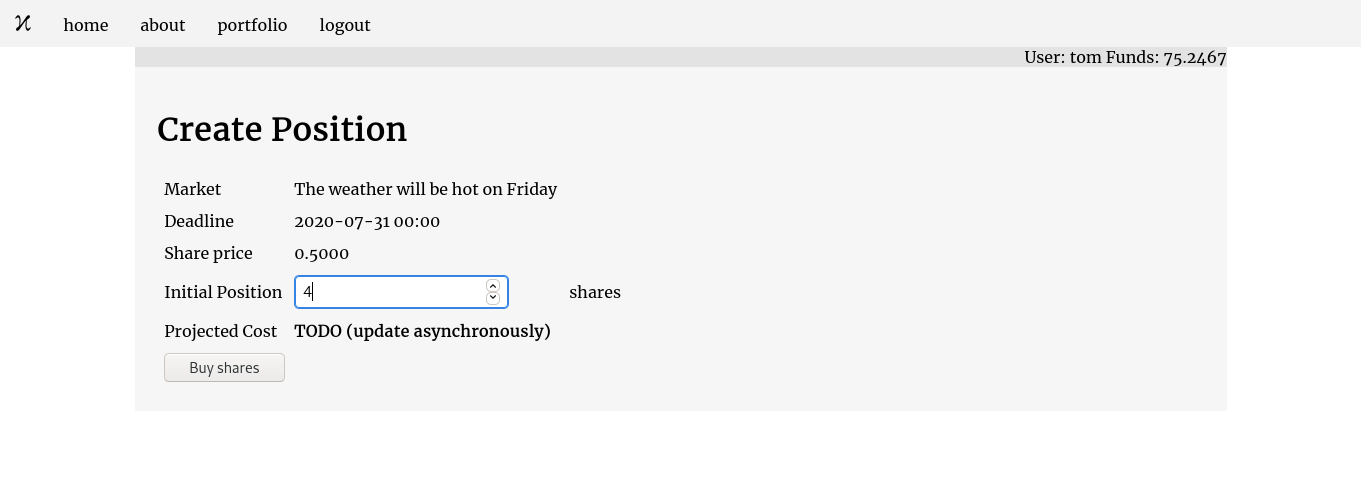
\includegraphics[width=.8\textwidth]{market-creation}
	\caption{Creating a market for the wager, ``The weather will be hot on
	Friday''}
	\label{fig:marketCreation}
\end{figure}

\subsubsection{Arbitration}

\label{sec:arbitration}

The arbitration stage of the mechanism seeks to resolve markets whose deadlines
have passed by gathering reports from arbiters and paying out, or demanding
money from, stakeholders. Since we will eventually be able to accommodate for
users to act as arbiters in market in which they themselves hold a position, we
allow any user to opt in to become an arbiter in an unresolved market.
Figure~\ref{fig:dashboard} shows the dashboard as it appears to a logged in
user, in which they are presented with all the currently active and unresolved
markets. 

\begin{figure}[h]
	\centering
	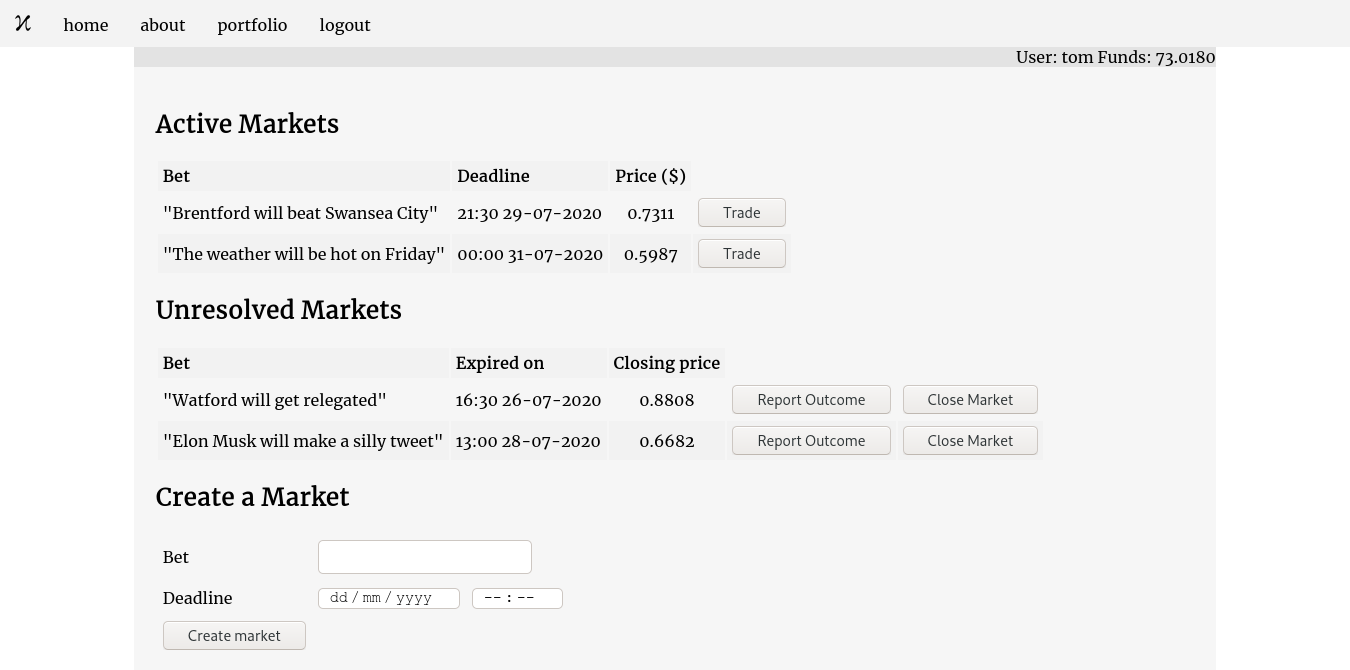
\includegraphics[width=.8\textwidth]{dashboard}
	\caption{A user's dashboard, where they can see all active and unresolved
	markets}
	\label{fig:dashboard}
\end{figure}

Once the user has opted in to arbitration they are taken to a form to submit
their report on the outcome, as well as estimations on their ``Positive
Belief'' and ``Negative Belief''. These are estimations of probabilities that,
given that the event \emph{actually} had a positive (respectively negative)
outcome, the user received a positive signal. This is important as we need to
take into account signal noise, given that wagers can be subjective: while the
positive and negative signal beliefs will be nearer to 1 and 0, respectively,
for an event such as the winner of a football match, since it will likely be
covered by many media outlets all reporting the true result, this may not
necessarily be the case where the outcome is more a matter of opinion. The
weakness of this approach is discussed in Section~\ref{sec:evaluation}.

\begin{figure}[h]
	\centering
	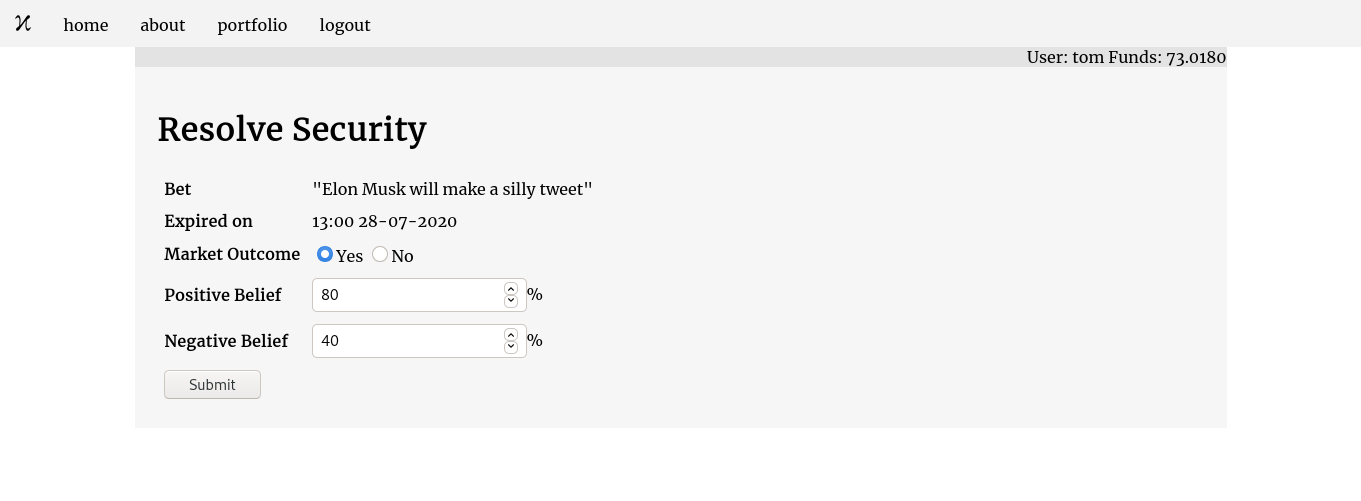
\includegraphics[width=.8\textwidth]{arbitration}
	\caption{The interface for submitting a report as an arbiter}
	\label{fig:resolveSecurity}
\end{figure}

These signal beliefs are used to compute the update probabilities $\mu_1$ and
$\mu_0$ which are used in the 1/prior-with-midpoint mechanism. Given the
closing price $\mu$ and the positive and negative signal beliefs
$\Pr[x_i=1|X=1]$ and $\Pr[x_i=1|X=0]$ for each arbiter $i$, we can compute the
positive update $\mu_1^i$ for each $i$ and randomly chosen $j$ as follows:
%
\begin{equation}
	\begin{aligned}
		\mu_1^i & = \Pr[x_j=1|x_i=1] \\
		& = \Pr[x_j=1|X=0] \cdot \Pr[X=0|x_i=1] + \Pr[x_j=1|X=1] \cdot
		\Pr[X=1|x_i=1]
	\end{aligned}
\end{equation}
%
We use the same approach to compute the negative update $\mu_0^i$ for each $i$,
and hence we may now also compute the common updates $\mu_1$ and $\mu_0$ to pay
arbiters the correct reward for arbitration. Once done, we set the outcome of
the market to the fraction of arbiters that reported a positive outcome, paying
users who hold shares and taking money from users that sold shares short.

\subsubsection{Server}

The code contained in \code{server.lisp} is responsible both for setting up and
maintaining the Hunchentoot web server and defining the various pages and forms
with which users interact.  Hunchentoot makes interaction with the web server
straightforward. We initialise the server by creating an \code{easy-acceptor},
and once we have defined our webpages using CL-WHO we simply push them to the
dispatch table using \code{create-prefix-dispatcher} so that they may be
accessed. Hunchentoot also provides us with automatic session handling, meaning
we do not have to worry about the details of logging in users on different
machines at the same time: we simply define the symbol \code{session-user} in
the appropriate session-handling data structure, then set this to the logged in
user. We can then access this using \code{(session-value 'session-user)} to
display different material on the page and interact with the database according
to the current user. Finally, we use Hunchentoot to access the GET and POST
parameters users send to the server via forms with a call to the library's
\code{parameter} function. 

Although there is little special to CL-WHO compared to other HTML-generating
libraries, it is useful to remain in the Lisp environment to define webpages
since we may use its powerful macro system. We use it to define a template for
a standard page, meaning we only need to specify the elements that make the
page unique and giving the web application a consistent style. This also
enables us to define pages and add the corresponding HTML generating function
to the dispatch table all within a single interface, hiding the unnecessary
details. Listing~\ref{lst:defineURL} shows how we are able to define both the
webpage, generate its content, and push it to the dispatch table in one.

The code in \code{server.lisp} draws together the interfaces from other areas
of the system and actually executes the mechanism. This involves taking user
input to create custom markets, quote share prices, and collect and distribute
payments for the various interactions users may have with the market.

\begin{lstlisting}[
	label={lst:defineURL},
	language=lisp,
	captionpos=b,
	caption={Defining webpages}]
(defmacro define-url-fn ((name) &body body)
  `(progn
     (defun ,name () ,@body)
     (push (create-prefix-dispatcher ,(format NIL "/~(~a~)" name) ',name)
           *dispatch-table*)))
\end{lstlisting}

\section{Project Management}

\label{sec:projectManagement}

\subsection{Methodology}

The project has been developed incrementally, with a focus on integrating new
functionality completely before progressing to new features. This approach is
well-suited to this project's design: since it comprises of mainly four
separate areas which are drawn together at the end, it is possible to focus on
implementing a feature within one area without it affecting the rest. As a
result, testing has been performed throughout and ensures that a newer version
of the project is never worse than its predecessor. Using Git and Github has
been helpful in this regard, providing cloud storage and the ability to roll
back to previous versions if the current one is broken by a new feature.

\subsection{Ethics}

There is little ethical consideration required for the development of this
project. All development and testing has been done independently, and all
resources used to implement the system is available freely. Testing has been
performed externally only to small extent, and even then only informally
through asking of colleagues' opinions. There is one ethical issue that faces
prediction markets in general, however, and the one we implement is no
exception. When prediction markets operate, directly or indirectly, with real
money, they run the risk of devolving into ``assassination
markets''~\cite{assassinationMarkets, crowdfundingMurder}. This refers to the
incentive that people may have to act in a way that changes the ``natural''
outcome of an event. In the extreme case, a bet may be made on the death of a
high-profile individual and an assassin could stand to make a large by
participating in the market and ensuring that the individual dies on a given
date. A way to sidestep this issue is to use virtual money with no real-world
value, and this is the approach we take.

\subsection{Scheduling}

There have been few issues regarding the scheduling of the project, though it
has benefited from a slight rearrangement of the initial timetable.
Figure~\ref{fig:old-schedule} shows the schedule as it was planned at the time
of the presentation, towards the start of the project's initial development.
Tasks have also taken slightly longer to implement, and a revised version is
given in Figure~\ref{fig:new-schedule}, which details both how time on the
project was spent and how we now plan to use the remaining time.

\begin{figure}[h]
	\centering
	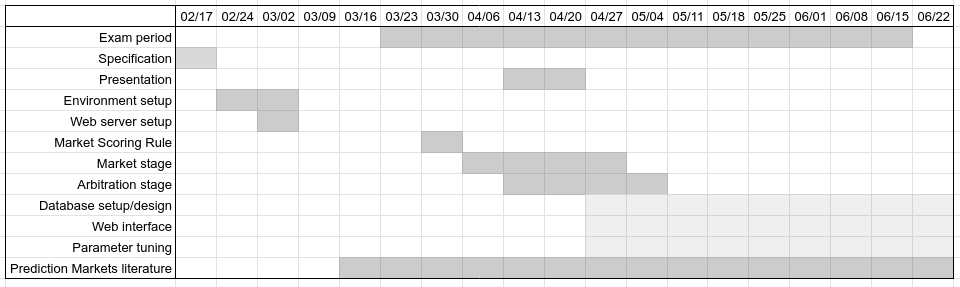
\includegraphics[width=\textwidth]{old-schedule}
	\caption{Project timetable as it was initially planned}
	\label{fig:old-schedule}
\end{figure}

Firstly, although an early demonstration of the market and arbitration stages
was complete for the presentation, this did not yet use any persistent storage
or actual users. Therefore, to get these stages working as they would in the
final project, the website and database interface first needed implementing.
This has taken the majority of the time since the presentation, and includes
defining the various pages and forms with which the users interact with the
markets, as well as how we interact with the database to register, log in, and
pay users. As we will cover in the next section, there are only three main
areas of functionality left to target: asynchronous communication with the
server via AJAX calls, automation of the system regarding closing markets once
enough arbiters have submitted reports, and most importantly parameter tuning.
The latter has been given a large block of time to complete since there are
many values on which certain parameters depend, and it is imagined that
calculating these accurately will require care.

Secondly, the time dedicated to writing the interim report has been extended by
two weeks to reflect the extension to its deadline. Although it was not
initially required, the extra time that could be diverted towards developing
the systems while the writing of the report was delayed was useful in providing
more material to discuss. This was also caused in part by more focus than
anticipated being paid towards exam preparation.

\subsection{Next Steps}

% Parameter tuning which requires processing of all data submitted 
% Asynchronous database queries to keep page details accurate

The next task is to tune the parameters of the system to ensure truthful
reporting, since this is the entire reason for implementing the mechanism. This
includes setting transaction fee $f$ to the appropriate percentage and the
payment parameter $k$. It will also be important to fully automate the system,
meaning the server automatically decides when to close markets: this is
currently done by prompting the system to compute market outcomes, which is
insufficient. The final important feature to add is asynchronous server
communication -- although it does not necessarily add new functionality to the
core of the prediction market, it would dramatically increase usability. 

We plan to dedicate a significant portion of August to the writing of the
dissertation, to spread the workload more evenly and to allow features that are
developed later more time to be added into the report.  We hope to get feedback
on a draft of the dissertation three weeks before the final deadline so that
the following weeks can be spent refining the material, and for more versions
to be produced in the remaining time. This means we intend to get all required
goals working well before the end of the month, to ensure we are not making
considerable changes shortly before the deadline.

\begin{figure}[h]
	\centering
	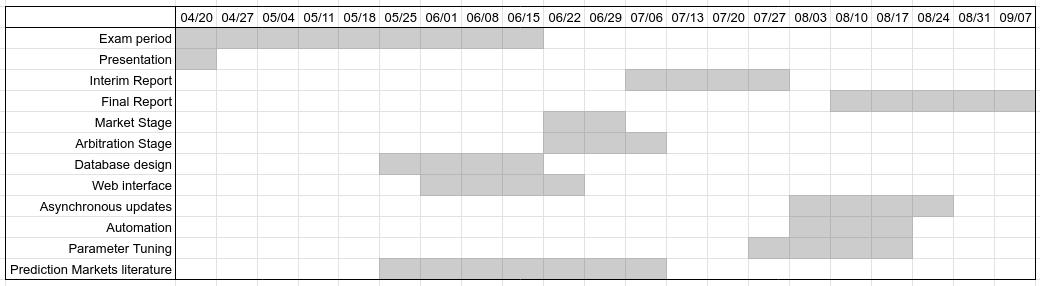
\includegraphics[width=\textwidth]{new-schedule}
	\caption{Revised project timetable}
	\label{fig:new-schedule}
\end{figure}

\section{Evaluation}

\label{sec:evaluation}

\subsection{Successes}

One main and obvious success of the project so far is that it successfully
implements a prediction market. This has required learning about the associated
game theory literature on mechanism design and scoring rules markets, and
although the project has taken a different shape since its proposal, a better
working knowledge on the current landscape of algorithmic game theory was
always a goal and has been achieved. An important point raised in the
presentation was that the project is not necessarily interesting because it
allows users to trade on predictions, but more so because it allows users to
create their own markets while remaining robust to manipulation, hence the game
theoretic, rather than strictly economic, approach.

The project has required learning the Lisp programming language having had no
prior experience in it. Writing custom macros to abstract away unnecessary
details in database interaction and HTML generation has provided particular
satisfaction.

\subsection{Improvements}

While there have been no particular failures of the project so far, there are
areas of it which can be improved. There is an issue of efficiency in database
access caused by an unfamiliarity with the Mito library. It is likely, however,
that we will not be able to rectify this in time, as it currently causes no
performance issues and there are more important tasks taking priority.

The frequency of supervisor meetings should be made more consistent as we
approach the final stages of the project. Until this point this has not been an
issue and was anticipated over the summer examination period, however as we
begin work on the final report a more steady opportunity to discuss problems
and receive feedback will become more useful. Although the irregularity of
meetings can be attributed in part to the remote working situation, the
facilities exist for meetings to be held remotely and should be used to a
greater degree as we approach the project's end.

There are also design aspects of the system that are worth improving. The
requirement for users to supply their estimates of signal accuracy is an issue:
it is unreasonable to ask for such estimations, and also opens up the
opportunity for users to manipulate the mechanism, which is the very behaviour
we wished to avoid. This is a weakness of the mechanism from Freeman et
al.~\cite{CODiPM}, and the issue arises as the signal posteriors are assumed to
be known by the system. In practice this is not possible since we have no way
of knowing the nature of where users get their signals. This problem could be
alleviated by calculating these probabilities based on past reporting and
market outcome histories, removing the interaction required from the user. It
would also be worth exploring the use of the Surrogate Scoring Rules introduced
by Liu et al.~\cite{Liu2020}, given that they do not need access to a ground
truth to score predictions. This could be particularly useful since a minor
issue of the mechanism we implement is that it is somewhat aged. This is not of
much concern, since no similar prediction market exists in a practical
implementation, however it would be interesting to improve on its shortcomings
using results and approaches from more recent works.

% Evaluation points
% - Ugly design pattern of `select-dao` then iterating with LISP (not SQL)
% - Not enough tutor meetings
% - Unrealistic to ask users to supply signal beliefs -- unlikely they know, but
% 	alternative is to have central person deciding on it and removing
% 	decentralisation
% - Too much processing code in server.lisp -- separate out into interfaces
% - Grace period? Time where no shares can be traded to prevent ambiguous
%   markets getting tanked by later investors
% TODO: eager loading in database

\bibliography{bibliography}

\begin{appendices}

%    \pagenumbering{gobble}
%
%    % timetable
%    \includepdf[landscape=true,pages=1,pagecommand={\section{Timetable}, \label{app:timetable}}]{timetable.pdf}
%    \includepdf[landscape=true,pages=2,pagecommand={}]{timetable.pdf}

\end{appendices}

\end{document}
